\documentclass[12pt]{article}
\usepackage{amsmath}
\usepackage{amsfonts}
\usepackage{fancyhdr}
\usepackage{titlesec}
\usepackage[margin=1in]{geometry}
\usepackage{siunitx}
\usepackage{booktabs}
\usepackage{graphicx}
\usepackage{float}
\usepackage[hidelinks]{hyperref}

\pagestyle{fancy}
\lhead{} 
\chead{} 
\rhead{\thepage} 
\lfoot{} 
\cfoot{} 
\rfoot{} 
\renewcommand{\headrulewidth}{0pt} 
\renewcommand{\footrulewidth}{0pt} 
%\titleformat{\section}[block]{\Large\bfseries\filcenter}{}{1em}{}
%\titleformat{\subsection}[block]{\large\bfseries\filcenter}{}{1em}{}
%To make sure we actually have header 0.5in away from top edge
%12pt is one-sixth of an inch. Subtract this from 0.5in to get headsep value
\setlength\headsep{0.333in}
\pagestyle{fancy}
\linespread{1.4}

\newcommand{\boldrule}{\rule{\linewidth}{2pt}} % Draws a thick line

\newcommand{\overbar}[1]{\mkern 1.5mu\overline{\mkern-1.5mu#1\mkern-1.5mu}\mkern 1.5mu} % Reduces length of \overline


\graphicspath{{Graphics/}}

\begin{document}

\thispagestyle{empty}
\newpage
\vspace*{3cm}
\begin{center}
%Lab title goes here
{\Huge EE 648 -- VLSI Design\\[.5cm]
Binary Coded Hexadecimal for a 7 Segment Display}
\end{center}
\vspace{5mm}
\boldrule\\
\begin{center}

\includegraphics{uaflogo.png}\\[.5cm]
\boldrule\\[3cm]
{\Large
\textsc{Ryker Dial}\\
\textsc{Cody Gossel}\\
\textsc{Zach Krehlik}\\[1cm]
February 17, 2017
}
\end{center}


\newpage

\thispagestyle{empty}
\tableofcontents

\newpage

\setcounter{page}{1}

%Rest of report goes here

\section{Introduction}
The goal of this project is to design and fabricate a chip that will use 4 input bits to control a 7 segment display. 
An integrated circuit such as this can be used to connect a 7 segment display to a microcontroller, reducing the number of output pins required to drive the display.
Four output pins of the controller are used to input the number to the IC, which then uses open collector outputs to pull down the cathodes of the 7 segment display. 


\section{Top Level Design}
The general strategy with the design is to separate the logic for each segment into its own module. 
Each module will be routed to an output pin through an open collector transistor to drive the 7 segment display. 
The top level diagram is shown in Figure \ref{fig:TopLevelCkt}.

\begin{figure}[h]
	\centering
	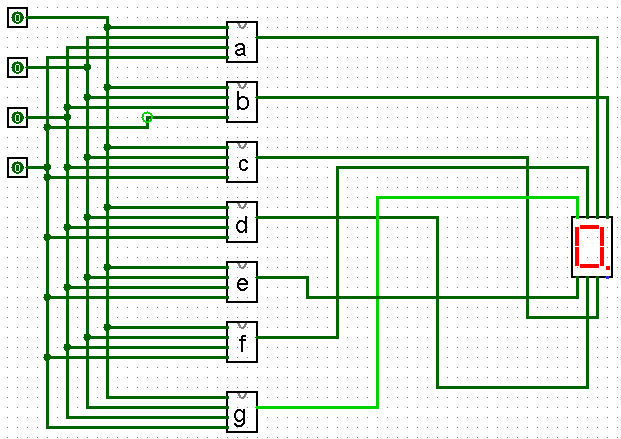
\includegraphics[scale=.8]{topLevelLogicCkt.png}
	\caption{Circuit top level layout}
	\label{fig:TopLevelCkt}
\end{figure}

Many of the gate level circuits use the inputs as well as their complements.  
To reduce the number of gates in the final design, the inputs will each be inverted before being to the logic circuitry.  
This will minimize redundancies in the gate layout.  
This has not been included in this iteration of the design.


\section{Detailed Design}
\subsection{Gate Level}

The truth table for the four inputs and all seven outputs was created, it is shown in Figure \ref{fig:truthTable}.

\begin{figure}[h]
	\centering
	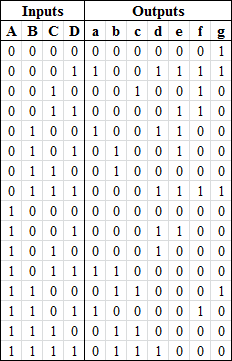
\includegraphics{hex7seg_truthTable.png}
	\caption{Circuit Truth Table}
	\label{fig:truthTable}
\end{figure}

The truth table was transferred to the free software Logisim one output at a time.  
Logisim analyzed the truth table for each output bit and generated a minimized NAND Boolean expression.  
Utilizing inverting logic will reduce the number of inverters required to realize the circuit.
Note that a zero in the output represents an active segment.
The equivalent set of logic equations is shown in Appendix \ref{app:logicEquations}.

Each logic equation represents a block on the top level diagram, and has a corresponding series of gates. The gate level design of these blocks is included in Appendix \ref{app:segmentLogic}.

\subsection{Transistor Level}

By optimizing the design to use only NAND gates the overall complexity is reduced. 
Efficient 2, 3, and 4 input NAND gates can be designed once and reused in block form.
Apart from the NAND gates, an inverter will also be required.
The transistor level design of these gates is shown in the figures below.

\begin{figure}[h]
	\centering
	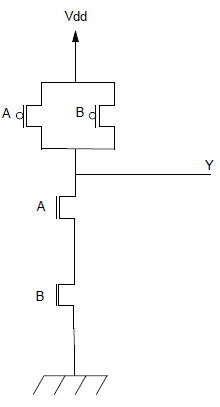
\includegraphics[scale=.5]{NAND_2_Trans.png}
	\caption{Circuit Truth Table}
	\label{fig:2nandTran}
\end{figure}

\begin{figure}[h]
	\centering
	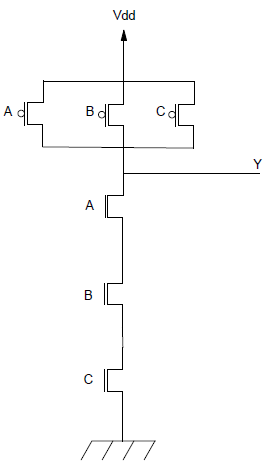
\includegraphics[scale=.5]{NAND_3_Trans.png}
	\caption{Circuit Truth Table}
	\label{fig:3nandTran}
\end{figure}

\begin{figure}[h]
	\centering
	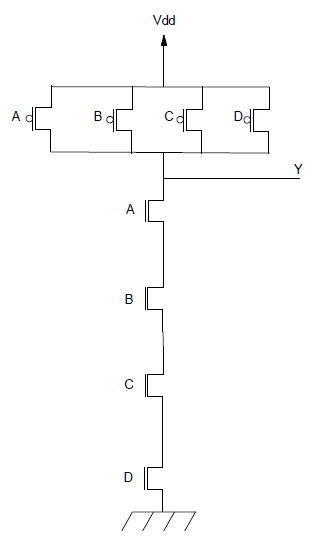
\includegraphics[scale=.5]{NAND_4_Trans.png}
	\caption{Circuit Truth Table}
	\label{fig:4nandTran}
\end{figure}

\begin{figure}[h]
	\centering
	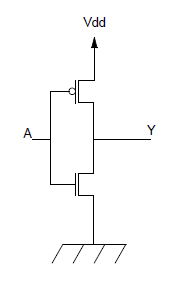
\includegraphics[scale=.5]{NOT_Trans.png}
	\caption{Circuit Truth Table}
	\label{fig:not}
\end{figure}



\newpage
\appendix
\section{Segment Logic Diagrams}
\label{app:segmentLogic}
% Segment a ==============================================
\subsection{Segment a}

\begin{figure}[H]
	\centering
	\label{fig:aBlockGates}
	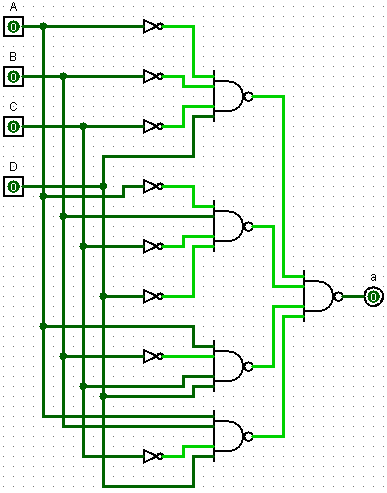
\includegraphics[width=0.5\linewidth, keepaspectratio]{a_logicCkt}
	\caption{Block a Gate Level Schematic}
\end{figure}

%Segment b ================================================
\subsection{Segment b}

\begin{figure}[H]
	\centering
	\label{fig:bBlockGates}
	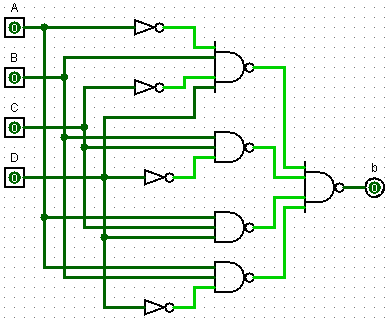
\includegraphics[width=0.5\linewidth, keepaspectratio]{b_logicCkt}
	\caption{Block b Gate Level Schematic}
\end{figure}

%Segment c ================================================
\subsection{Segment c}
\begin{figure}[H]
	\centering
	\label{fig:cBlockGates}
	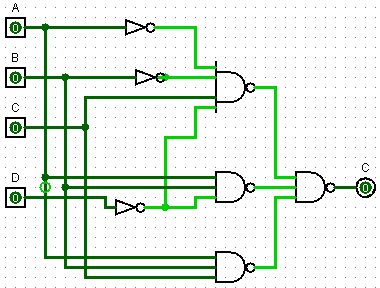
\includegraphics[width=0.5\linewidth, keepaspectratio]{c_logicCkt}
	\caption{Block c Gate Level Schematic}
\end{figure}

%Segment d =================================================
\subsection{Segment d}
\begin{figure}[H]
	\centering
	\label{fig:dBlockGates}
	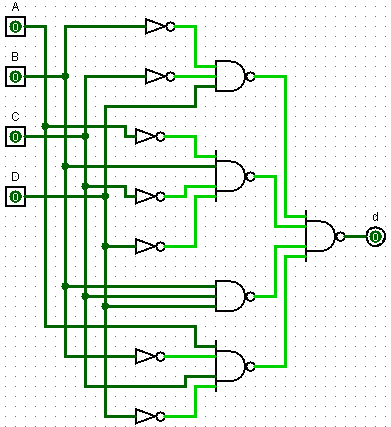
\includegraphics[width=0.65\linewidth, keepaspectratio]{d_logicCkt}
	\caption{Block d Gate Level Schematic}
\end{figure}

%Segment e ================================================
\subsection{Segment e}
\begin{figure}[H]
	\centering
	\label{fig:eBlockGates}
	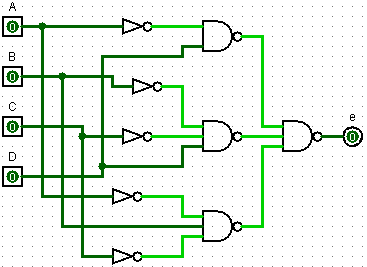
\includegraphics[width=0.65\linewidth, keepaspectratio]{e_logicCkt}
	\caption{Block e Gate Level Schematic}
\end{figure}

%Segment f ================================================
\subsection{Segment f}
\begin{figure}[H]
	\centering
	\label{fig:fBlockGates}
	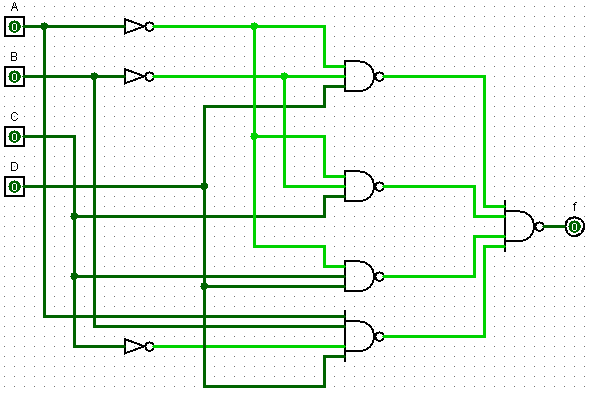
\includegraphics[width=0.65\linewidth, keepaspectratio]{f_logicCkt}
	\caption{Block f Gate Level Schematic}
\end{figure}

%Segment g ================================================
\subsection{Segment g}
\begin{figure}[H]
	\centering
	\label{fig:gBlockGates}
	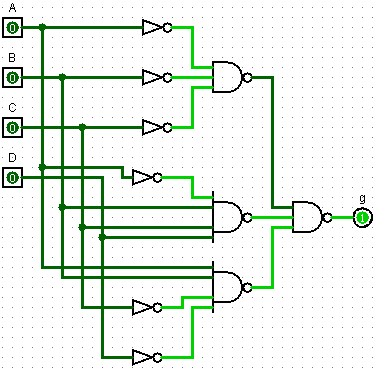
\includegraphics[width=0.65\linewidth, keepaspectratio]{g_logicCkt}
	\caption{Block g Gate Level Schematic}
\end{figure}


\newpage
\section{Logic Equations}
\label{app:logicEquations}
\begin{equation}
a = \overline{\overbar{(\bar{A}\bar{B}\bar{C}D)}\overbar{(\bar{A}B\bar{C}\bar{D})}\overbar{(A\bar{B}CD)}\overbar{(AB\bar{C}D)}}
\end{equation}

\begin{equation}
b = \overline{\overbar{(\bar{A}B\bar{C}D)}\overbar{(BC\bar{D})}\overbar{(ACD)}\overbar{(AB\bar{D})}}
\end{equation}

\begin{equation}
c = \overline{\overbar{(\bar{A}\bar{B}C\bar{D})}\overbar{(AB\bar{D})}\overbar{(ABC)}}
\end{equation}

\begin{equation}
d = \overline{\overbar{(\bar{B}\bar{C}D)}\overbar{(\bar{A}B\bar{C}\bar{D})}\overbar{(BCD)}\overbar{A\bar{B}C\bar{D}}}
\end{equation}

\begin{equation}
e = \overline{\overbar{(\bar{A}D)}\overbar{(\bar{B}\bar{C}D)}\overbar{(\bar{A}B\bar{C})}}
\end{equation}

\begin{equation}
f = \overline{\overbar{(\bar{A}\bar{B}D)}\overbar{(\bar{A}\bar{B}C)}\overbar{(\bar{A}CD)}\overbar{(AB\bar{C}D)}}
\end{equation}

\begin{equation}
g = \overline{\overbar{(\bar{A}\bar{B}\bar{C})}\overbar{(\bar{A}BCD)}\overbar{(AB\bar{C}\bar{D})}}
\end{equation}


\end{document}
